\documentclass{beamer}
\usetheme{default}
\hypersetup{
    colorlinks=true,
    linkcolor=blue,
    urlcolor=cyan
}

\title{Temoc Offensive}
\subtitle{A temoc- and space- themed shooter}
\author{Team 15: Ethan Usrey, Daniel Yahalom, Agastya Bose, Timothy Sweet}
\institute{The University of Texas at Dallas}
\date{\today}

\begin{document}

\begin{frame}
\titlepage
\end{frame}

\section{Game Overview}
\subsection{Introduction}

\begin{frame}
\frametitle{Introduction}
    \begin{columns}
        \column{0.5\textwidth}
    \begin{itemize}
        \item Our game is a space-themed player-vs-player first-person shooter.
        \item It takes place on a small space station built on an asteroid, and the players are temoc-like astronauts.
        \item It supports online multiplayer.
    \end{itemize}
        \column{0.5\textwidth}
        \begin{figure}
            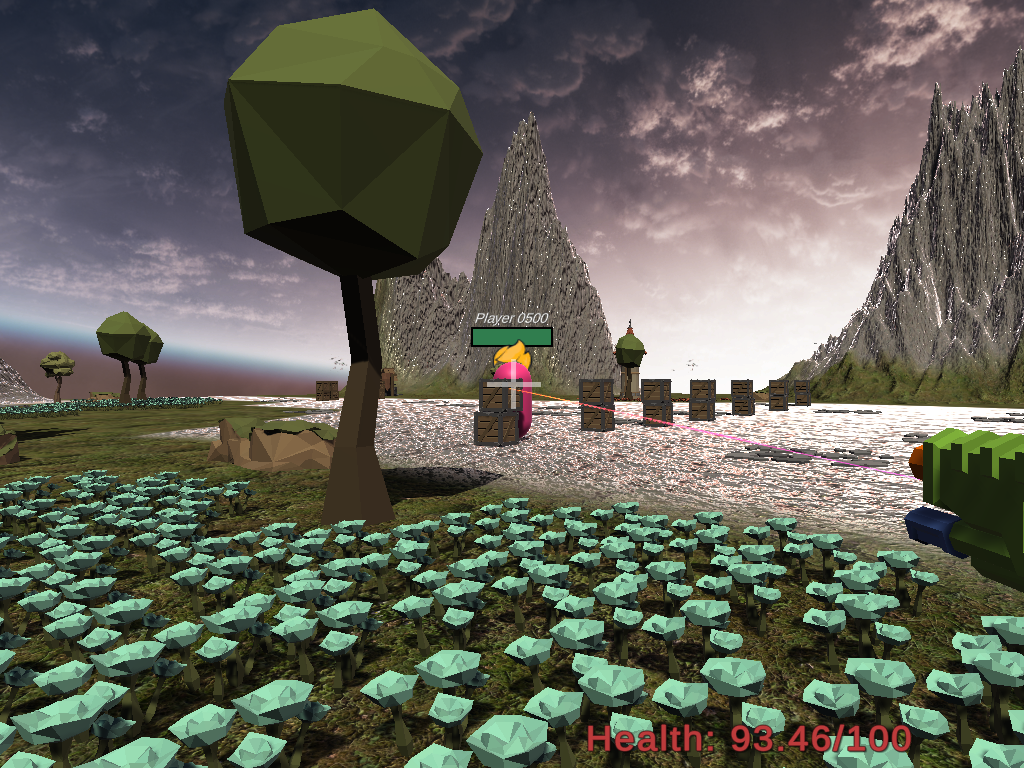
\includegraphics[width=\textwidth]{being_shot_at}
            \caption{The player being shot at by the astronaut with Temoc hair}
        \end{figure}
    \end{columns}
\end{frame}

\subsection{Gameplay Mechanics}

\begin{frame}
\frametitle{Gameplay Mechanics}
Upon launching the game, players can create or join an online lobby, upon which they will spawn on the map. When a player shoots another player, the target's health will drain, and when it runs out, they will respawn at the original spawn point.

Controls:

    \begin{itemize}
        \item WASD or Arrow keys - move
        \item Space - jump
        \item Shift - sprint
        \item Mouse cursor - move viewport
        \item Mouse button 1 - shoot laser
        \item Mouse button 3 - shoot rocket
    \end{itemize}

\end{frame}

\subsection{Design}

\begin{frame}
\frametitle{Design}
The game takes place in a small base built on an asteroid. The map consists primarily of rocky hills, with some evidence of the players living there, such as small trees, buildings, and boxes. The playable characters are Temocs in pill-like astauronaut suits. The players' guns shoot lasers and rockets.

    \begin{figure}
        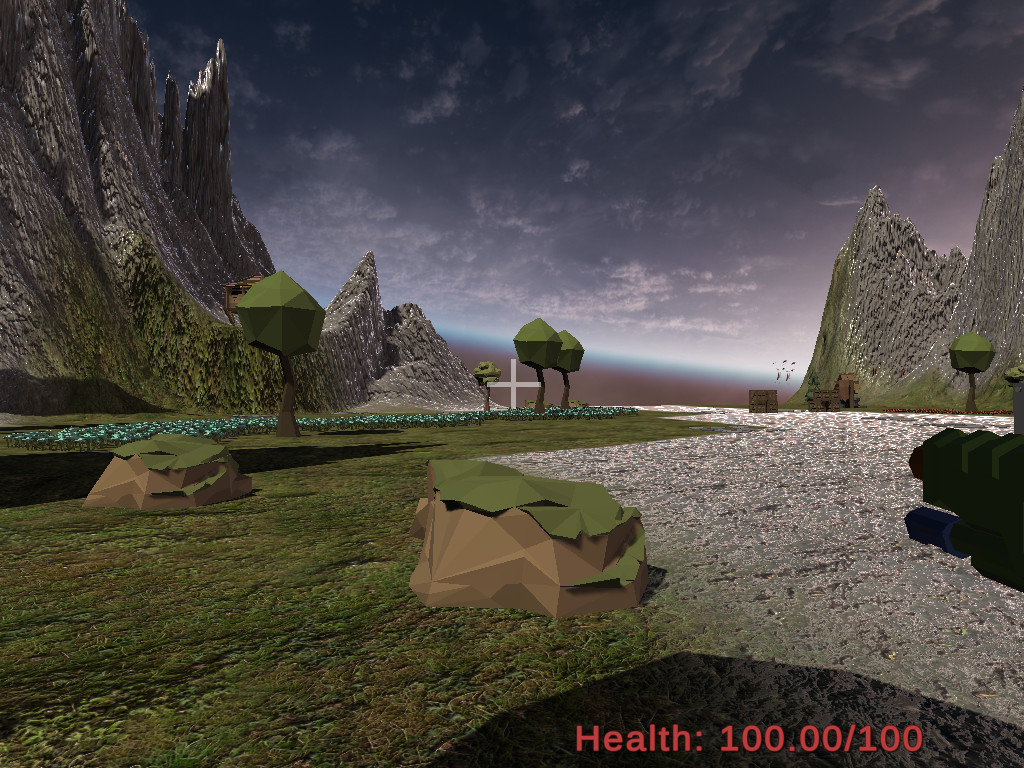
\includegraphics[height=0.5\textheight,keepaspectratio]{scenery}
        \caption{The game's scenery}
    \end{figure}

\end{frame}

\section{Technical Details}

\subsection{Software Used}
\begin{frame}
\frametitle{Software Used}
This game was built in Unity. We used some of Unity's free texture pack along with Blender for creating the models for the map and players.

    \begin{figure}
        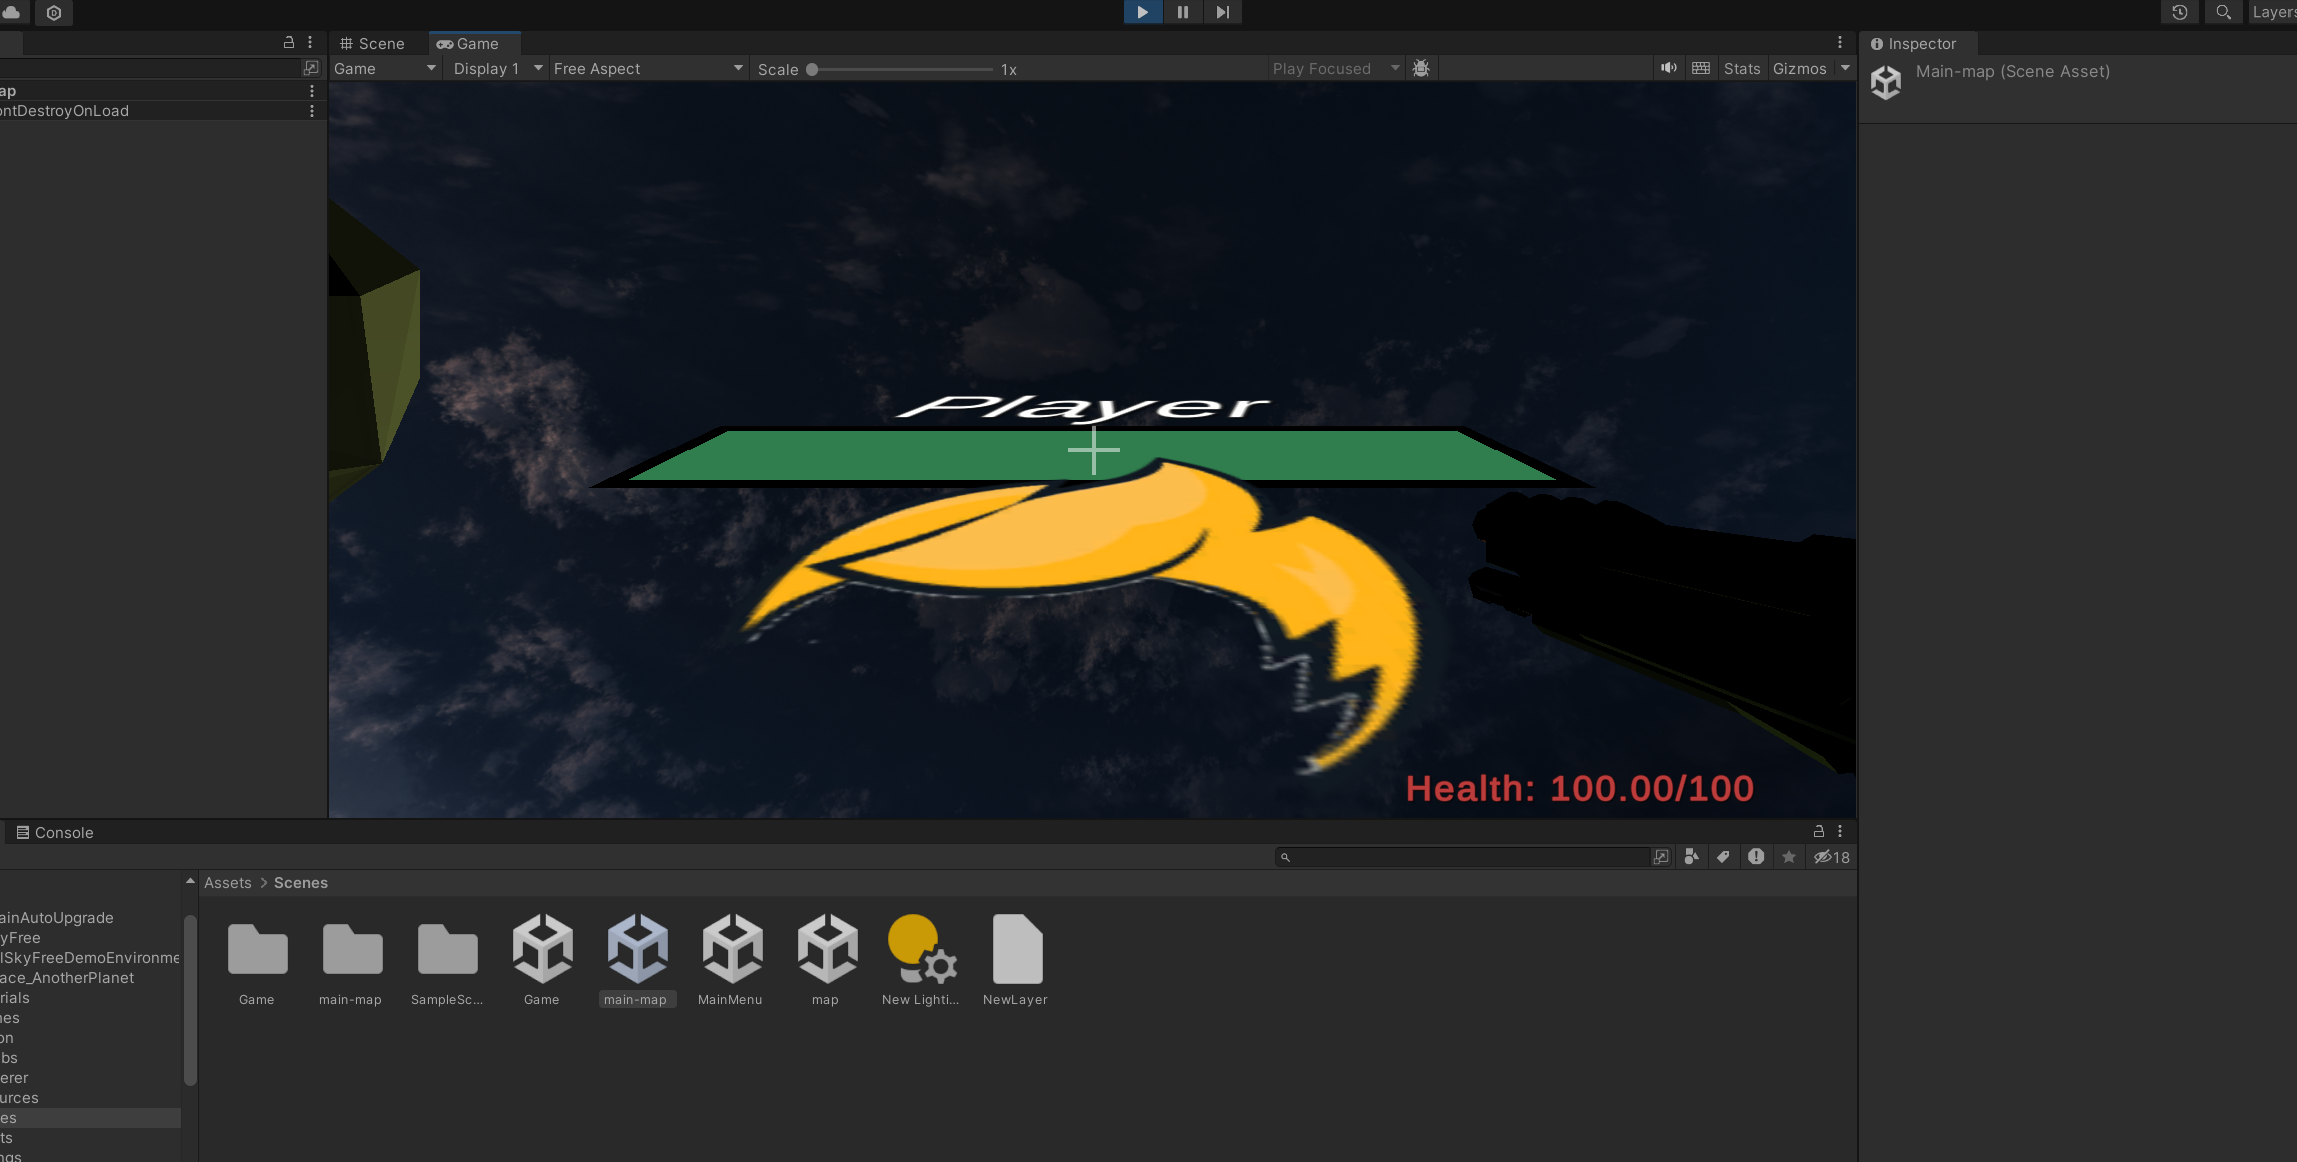
\includegraphics[width=\textwidth,keepaspectratio]{unity}
        \caption{Unity Editor}
    \end{figure}

\end{frame}

\subsection{Implementation Details}
\begin{frame}
\frametitle{Implementation Details}

    \begin{figure}
        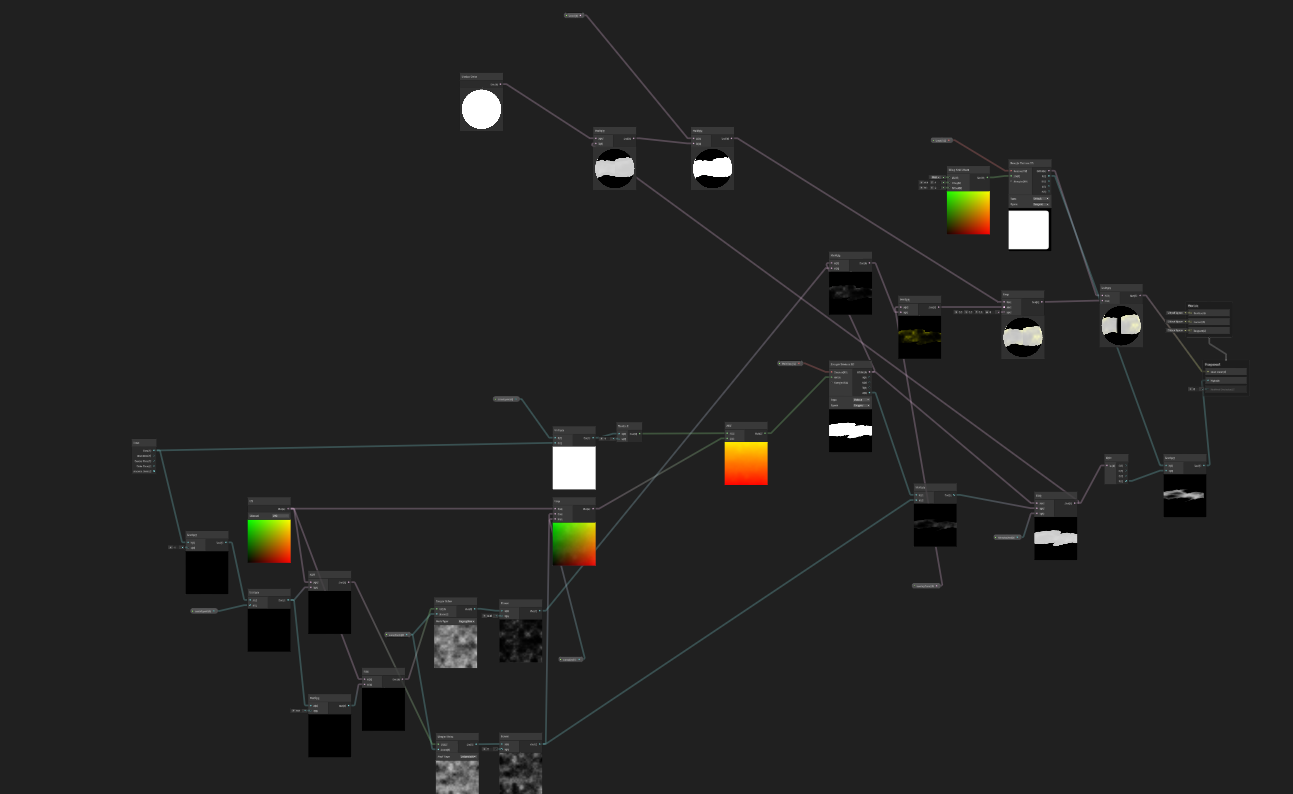
\includegraphics[width=\textwidth,keepaspectratio]{shader_graph}
        \caption{The shader graph for the laser}
    \end{figure}

\end{frame}

\begin{frame}
\frametitle{Implementation Details}

    \begin{columns}
        \column{0.5\textwidth}
    \begin{figure}
        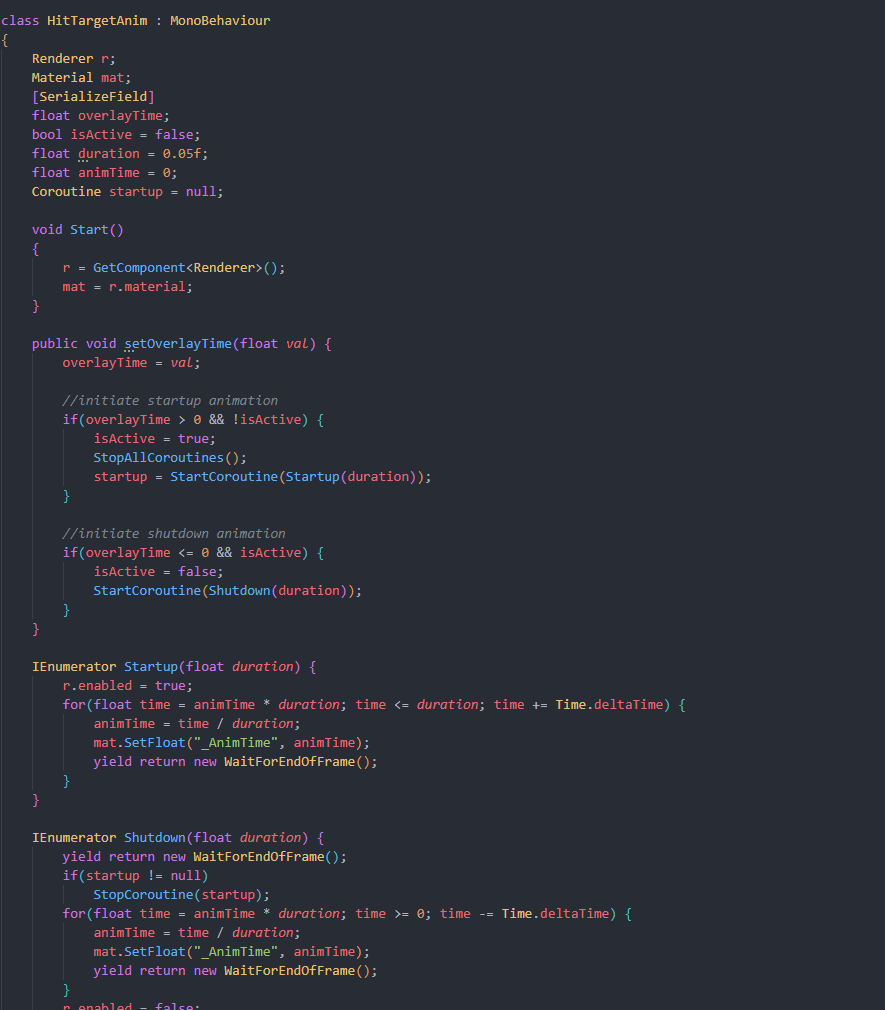
\includegraphics[width=\textwidth,keepaspectratio]{animations_scripting}
        \caption{Controlling animatins through scripting}
    \end{figure}
        \column{0.5\textwidth}
        \begin{figure}
            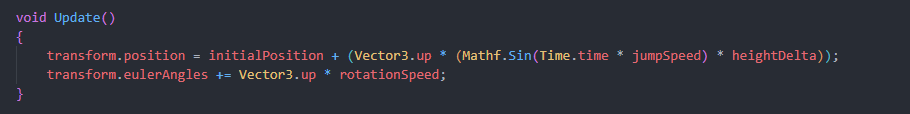
\includegraphics[width=\textwidth,keepaspectratio]{update}
        \end{figure}
    \end{columns}


\end{frame}

\subsection{Development Tools Used}
\begin{frame}
\frametitle{Development Tools Used}
In addition to Unity Editor, we used Visual Studio Code for the development, and tracked our changes in Git for collaboration.
\end{frame}

\subsection{Asset Packs Used}
\begin{frame}
\frametitle{Asset Packs Used}
    \begin{itemize}
        \item \href{https://assetstore.unity.com/packages/2d/textures-materials/nature/terrain-textures-pack-free-139542}{Terrain Textures Pack Free}
        \item \href{https://assetstore.unity.com/packages/2d/textures-materials/sky/allsky-free-10-sky-skybox-set-146014}{AllSky Free - 10 Sky / Skybox Set}
        \item \href{https://assetstore.unity.com/packages/3d/environments/polygon-sampler-pack-207048}{Polygon Sampler Pack}
    \end{itemize}
\end{frame}

\section{Development Status}

\subsection{Current Status}
\begin{frame}
\frametitle{Current Status}
    \begin{itemize}
        \item We have implemented a main menu system as our UI
        \item The game supports multiplayer battles through Photon
        \item You can find existing online rooms, create a room, or quit the game (please never quit playing our game)
        \item Upon joining a room, you are placed in a fairly large map with details such as trees, mountains, and some props
        \item The player can move around and discharge their weapons on other players in the world
        \item Currently implemented: a laser gun and a rocket launcher
        \item Laser gun has particle effects
    \end{itemize}
\end{frame}

\subsection{Challenges Faced}
\begin{frame}
\frametitle{Challenges Faced}
    \begin{columns}
        \column{0.5\textwidth}
    \begin{itemize}
        \item Two of us have never done game development nor worked with 3D modeling ever before. Learning even basic usage of immensely complex software like Blender was difficult.
        \item The textures were gigantic and could not be uploaded to GitHub, so we had to use catbox and cloud storage to send it them to each other.
    \end{itemize}
        \column{0.5\textwidth}
        \begin{figure}
            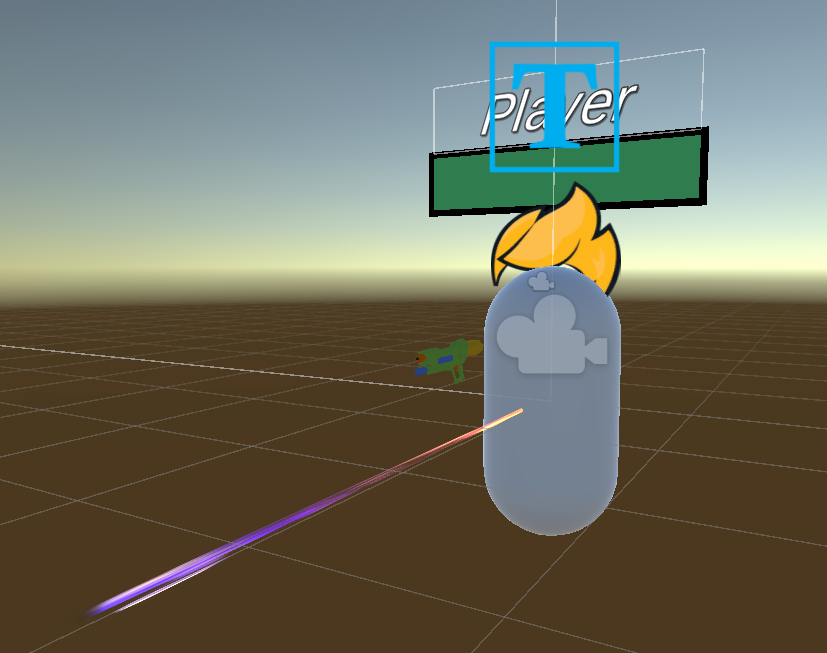
\includegraphics[width=\textwidth,keepaspectratio]{glitched_player}
        \end{figure}
    \end{columns}
\end{frame}

\subsection{Future}
\begin{frame}
\frametitle{Future}
We have many ideas and plans to improve our game from here, including:
    \begin{itemize}
        \item Implement sound (this is a graphics class so sound wasn't our priority)
        \item Make more maps (and more detailed maps)
        \item Make more detailed character models
        \item More weapons
        \item Give the rockets a trail 🚀
        \item Improve the UI
        \item Include in-game tutorial
        \item Implement particle fx (explosions, laser burns)
    \end{itemize}

\end{frame}

\section{Live Demonstration}

\begin{frame}
\frametitle{Live Demonstration}
    It is time for a live demonstration! You can join the game! Linux and Windows builds are available for download at \href{https://utdallas.box.com/s/q7e6fjieyb50r23selvv29iurs2q6z3z}{https://utdallas.box.com/s/q7e6fjieyb50r23selvv29iurs2q6z3z}. This link has also been posted in the class Discord server.
\end{frame}

\section{Questions?}

\begin{frame}
\frametitle{Questions?}
\end{frame}


\end{document}


